\documentclass{article}
\usepackage{amsmath,amssymb,amsthm, graphicx, float}
\usepackage{mathpazo}
\author{Alexandre Vassalotti \quad \'{E}ric Renaud-Houde}
\title{COMP 558: Final Project Report \\
  \large \textbf{Surface reconstruction using the level set method}
}
\date{27 April 2012}

\begin{document}
\maketitle
\section{Introduction}
Modelling surfaces from unorganized set of points, or point clouds, is a long
standing problem in the computer vision community. Indeed, problem is known to
be very challenging in three and higher dimensions. Furthermore, the problem
is ill-posed which means there is not a unique solution. When the point cloud
is dense enough and the topology of the surface is not complicated, a simple
solution could be to perform a Denaulay triangulation of points, like
described by Boissonnat \cite{boissonnat1984geometric}. However, even in this
context ambiguities can arises and lead to non desirable surface
reconstructions.

A desirable reconstruction method should be able to deal with irregularities
caused by noise and non-uniformity of the data collected. It should also be
able to deal with complex surface topologies as well. In addition, the
reconstructed surface should be representative of the point cloud. It should
be reasonably smooth yet maintain discontinuities.

Many approaches have been proposed to solve the surface reconstruction
problem. In general, the solutions can be categorized by the surface
representation they use---i.e, explicit or implicit. In an explicit
representation, the location of all the points on the surface is described
precisely. Triangulations methods yield such representations. Conversely, in
an implicit representation, we describe the surface as a constraint in a
higher dimension, or 3D space in our case. Implicit representations are often
advantageous because they lead to solutions capablable of handling complex
topologies. Their main drawback is they tend to be more expensive in time and
space.

Level-set methods are a class of techniques working on implicit
representations. These methods were developed conjointly by Osher and Sethian
\cite{sethian1999level}

With the arrival of low-cost depth sensors, such as the Microsoft's Kinect,
the opportunities for object and scene reconstruction are obvious. These depth
sensors provide accurate and dense measurements. A caveat however is these new
devices are typically structured light sensors. And the data from such devices
have large holes due to the shadows casted by the objects being measured. This
poses extras challenges for surfaces reconstruction.


\begin{figure}
  \centering
  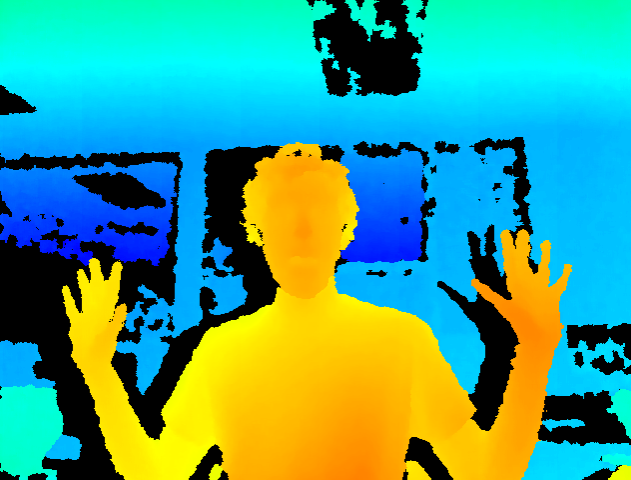
\includegraphics[width=0.7\textwidth]{img/depthmap.png}
  \caption{In this depth image taken using Microsoft's Kinect sensor, we see
holes, represented as black regions, where the sensor couldn't take
measurements.}

\end{figure}


\section{Framework}

Definitions:
\begin{itemize}
\item $\mathcal{S}$ : Data set of points.
\item $\Gamma$ : Level set embedded in $\phi$ (a contour curve in 2d or an
    isosurface in 3d).
\item $\phi$ : Implicit level set function (the evolving higher dimensional
    interface also called hypersurface).
\end{itemize}

\paragraph{Discretization}

Given that the surface motion equation for $\phi$ is defined as a partial
differential equation, we can solve it using iterative schemes for PDEs. As most
differential equations which might appear fairly innocuous at first, solving
them numerically can be quite challenging.

Given an initial value $\phi_0$, our first intution might be to apply the
first-order Euler method as follows:
\begin{align}
  \frac{\partial \phi}{\partial t} + F \|\nabla \phi\| &= 0 \\
  \frac{\phi^{t+1} - \phi^{t}}{\Delta t} &=  -F \|\nabla \phi\| \\
  \phi^{t+1} &= \phi^{t} - \Delta t \; F \|\nabla \phi\| 
\end{align}

However, not only does the Euler method often suffers from stability problems,
it is used in the context of \textit{ordinary differential equations}, not PDEs.
In that case, a different numerical procedure is needed. 

\subparagraph{Upwind Scheme}
One approach for discretizing PDEs, originally defined by Couran, Isaacson and
Rees \cite{courant1952solution} is called the upwind scheme. Instead of using
central differences for computing the partial derivatives, it uses both a
forward or a backward difference:

\begin{align}
    \frac{\partial p}{\partial x}^{-} &= p^{-}_x = \frac{p_i -
    p_{i-1}}{ \Delta x} = p_i - p_{i-1} \\
    \frac{\partial p}{\partial x}^{+} &= p^{+}_x = \frac{p^{i+1}_x -
    p^i_x}{ \Delta x} = p^{i+1}_x - p^i_x  
\end{align} since $ \Delta x = 1 $ in our grid. The same applies for other axes
$y$ and $z$.

\begin{figure}[htb]
  \centering
  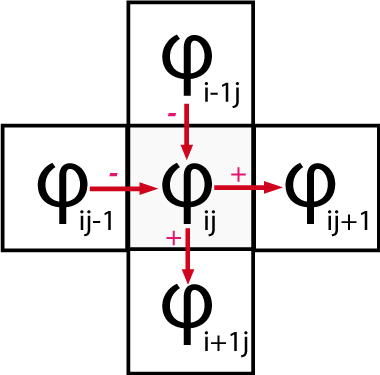
\includegraphics[width=0.45\textwidth]{img/upwind_grid.png}
  \caption{Illustration of the forward and backward differences over a 2d grid.}    
\end{figure}


Later used by Sethian\cite{sethian1999level} \cite{sethian1999advancing} for
the initial value formulation, he defines the classical level set method as
follows (let $ p = \phi_{ijk}$):

\[
p^{n+1} = p^{n} - \Delta t [ \max(F_{ijk}, 0) \| \nabla p \|^{+} + \min(F_{ijk},
0) \| \nabla p \|^{-} ]
\]
where:
\begin{align}
    \| \nabla p \|^{+} & = 
    \begin{bmatrix}
        \max(p^{-}_x, 0)^2 + \min(p^{+}_x, 0)^2 + \\
        \max(p^{-}_y, 0)^2 + \min(p^{+}_y, 0)^2 + \\
        \max(p^{-}_z, 0)^2 + \min(p^{+}_z, 0)^2
    \end{bmatrix}^{1/2}  \\
    \| \nabla p \|^{-} & = 
    \begin{bmatrix}
        \max(p^{+}_x, 0)^2 + \min(p^{-}_x, 0)^2 + \\
        \max(p^{+}_y, 0)^2 + \min(p^{-}_y, 0)^2 + \\
        \max(p^{+}_z, 0)^2 + \min(p^{-}_z, 0)^2
    \end{bmatrix}^{1/2} 
\end{align}

Rewriting this equation in terms of the entire grid matrices, and defining
$\odot$ as element-wise matrix mutiplication, we have the following formulation
which updates our entire grid for $\phi$:
\[
\phi^{n+1} = \phi^{n} - \Delta t [ \max(F, 0) \odot \| \nabla \phi \|^{+} +
\min(F, 0) \odot \| \nabla \phi \|^{-} ]
\]

As opposed to computing the magnitude of the gradient using the central
differences functions, the evolution of $\phi$ under the upwind scheme is much
more stable. Note that there are higher-order schemes listed in
\cite{sethian1999level} if more stability is required.

\begin{figure}[H]
  \centering
  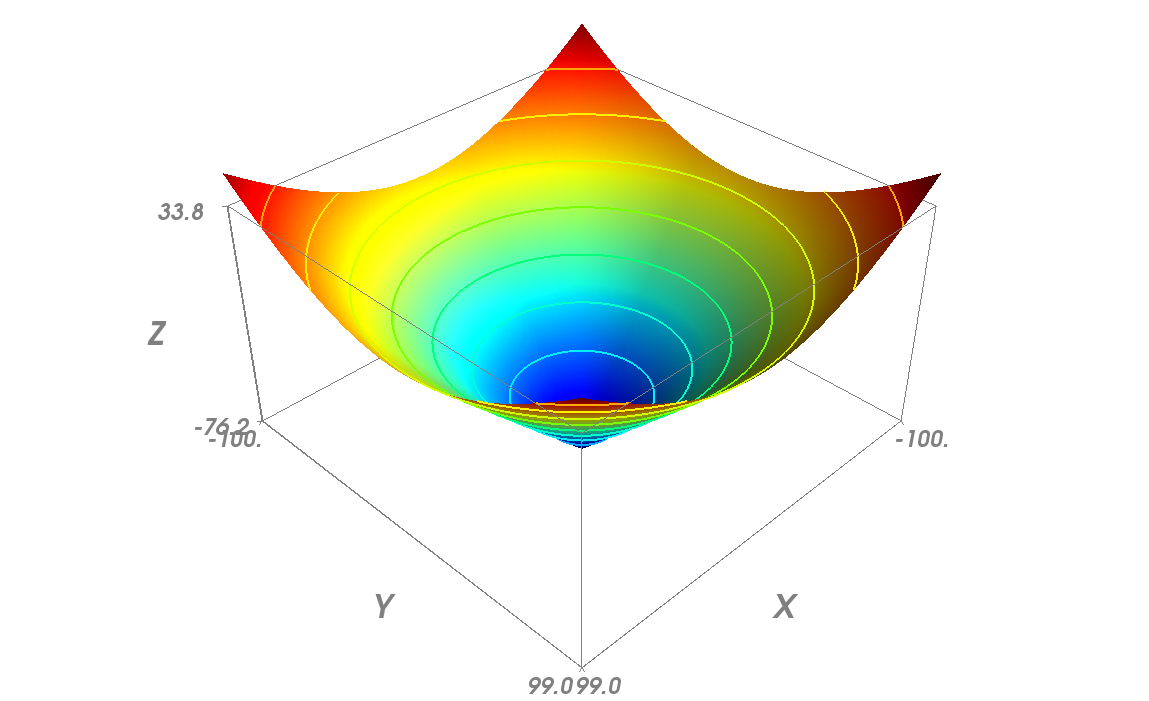
\includegraphics[width=0.8\textwidth]{img/up01.png}
  \caption{Initial hypersurface $\phi$ defined as a signed distance function
  (for a level set in 2d).}    
\end{figure}

\begin{figure}[H]
  \centering
  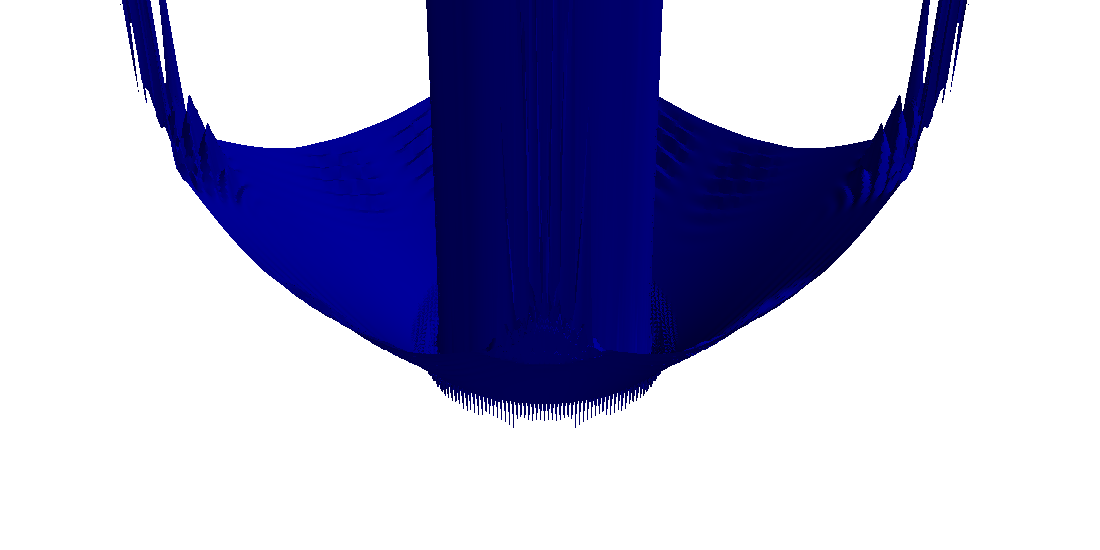
\includegraphics[width=0.8\textwidth]{img/up03.png}
  \caption{Result of 140 iterations using $\Delta t = 0.5$ and a constant force
  of 1 using the central differences approximations. The resulting hypersurface
  has exploded in the center and near the borders.}    
\end{figure}

\begin{figure}[H]
  \centering
  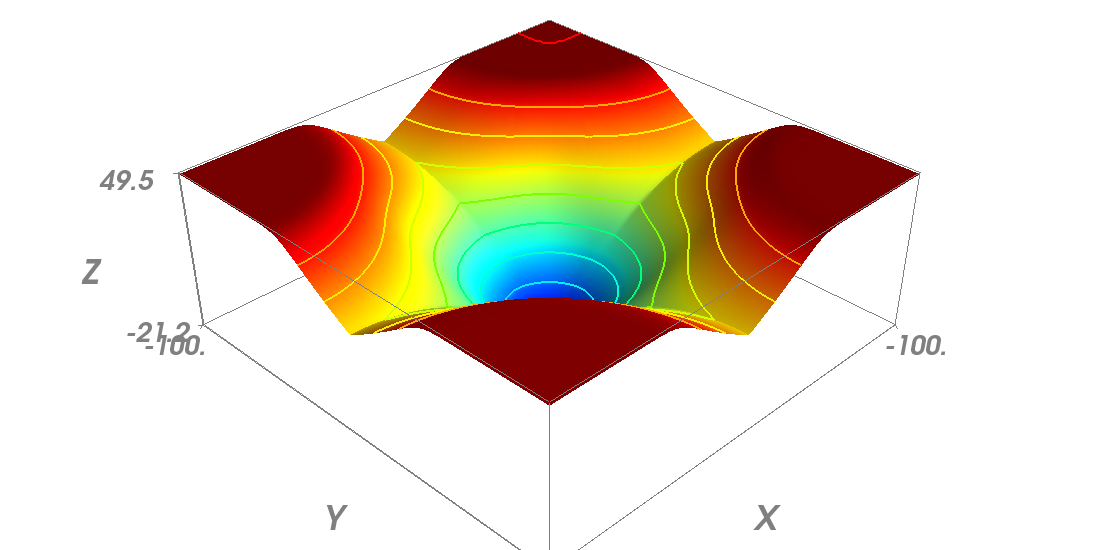
\includegraphics[width=0.8\textwidth]{img/up02.png}
  \caption{Result of 140 iterations using $ \Delta t = 0.5$ and a constant force
  of 1 using the upwind scheme. The hypersurface evolution is perfectly stable.
  It ultimately flattens out and remains so.}    
\end{figure}

\subparagraph{Implementation}
To implement the upwind scheme for the entire grid
update, a few strategies can be used. In the contex of matlab or numpy, it is
recommended to compute forward and backward differences using entire rows at
once. Also note that only one matrix is needed to store the results because the
squared differences can be added on top of each other.  Furthermore for the
edges of the grid, the inward row/column should be used in replacement if the
difference exceeds the matrix.

\paragraph{Forces governing surface evolution}
Up until now, we have left one variable undefined, namely the force matrix $F$.
The definition of this term very much depends on the application of the
algorithm. For example, a popular approach used in 2d segmentation (for example
in the context of medical imagery) is to employ (the magnitude of) gradients of
the image to limit the evolution of the level. However with a pointcloud, the
force must be derived differently. A formulation was specifically developped by
Zhao in \cite{zhao1} and \cite{zhao2001fast} for shape reconstruction from an
unorganized dataset of points.

Stating his formulation upfront, we have:
\[
F = \nabla d(\mathbf{x}) \cdot \frac{\nabla \phi}{\| \nabla \phi \|}
+ d(\mathbf{x}) \cdot (\nabla \cdot \frac{\nabla \phi}{\| \nabla \phi \|} )
\]
where $d(\mathbf{x})$ is an unsigned distance function to the closest point in
our dataset $S$.

The role of this force is twofold: it simultaneously encourages smoothness in
the level set and close fit to the data points which are attracting it.

\subparagraph{Energy Functional}
Where does this force formulation comes from? Derived from energy functional
$E(\Gamma)$.
\begin{itemize}
% Think of an elastic membrane
%attraction to points, push against high-curvature regions in the data
\item Quantifies how $\Gamma$ corresponds to the data set, with a smoothness
    constraint
\item Has two global minima: $\Gamma = \Gamma_0$  and $\Gamma = \emptyset$.
\end{itemize}
It can be shown that the minimizer of the functional satisfies:
\[
\nabla d(\mathbf{x}) \cdot \mathbf{n} + d(\mathbf{x}) \cdot \kappa = 0
\]
Note that the level set can reach a local minimum easily if the initial value
was not close enough to the final surface. As such, it is expected that this
methods results in some loss of details.
\begin{figure}[H]
  \centering
  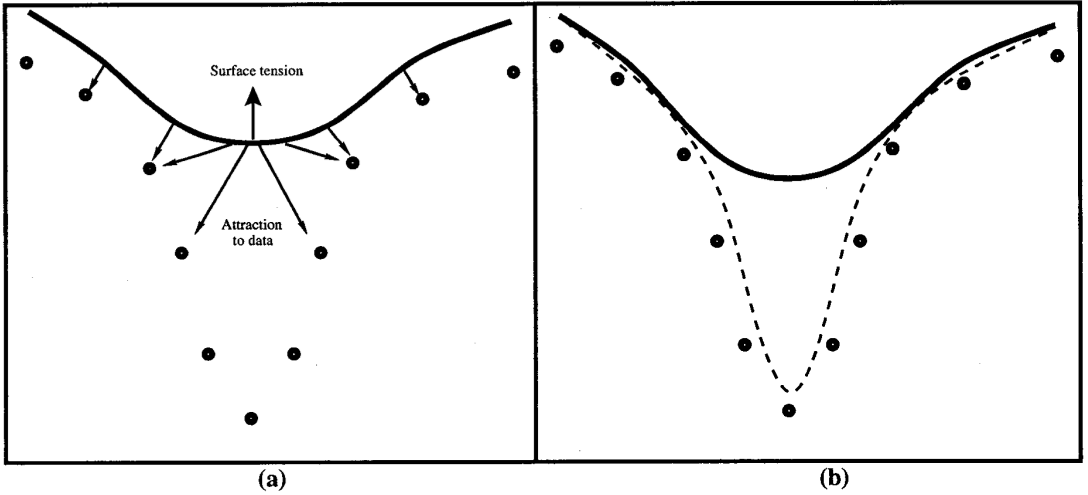
\includegraphics[width=1.0\textwidth]{img/savadjiev3_3.png}
  \caption{This figure taken from \cite{savadjiev2003surface} illustrates
  how the level set might be unable to reach the bottom of a crevasse. The local
  minumum (b) is reached from (a). The surface tension prevents the curve from
  bending and lower points cannot attract the surface further down because they
  are not the closest.}    
\end{figure}

\bibliographystyle{amsplain}
\bibliography{vision}

\end{document}
